\documentclass[titlepage]{article}
\usepackage[utf8]{inputenc}
\usepackage{fancyhdr}
\usepackage{titling}
\usepackage{tabto}
\usepackage[ddmmyyyy]{datetime}
\usepackage{graphicx}
\renewcommand{\dateseparator}{.}
\renewcommand{\figurename}{Obr.}
\renewcommand{\contentsname}{Obsah}
\graphicspath{ {/home/andras/Documents/kop/img/} }
\title{\textbf{Jednozvodový elektrokardiograf} \\
\large Praktická časť odbornej zložky maturitnej skúšky}
\date{\empty}

\begin{document}

\bgroup
	\fancypagestyle{empty} {
		\fancyhead[C] {Stredná priemyselná škola elektrotechnická S. A. Jedlika v Nových Zámkoch}
		\fancyfoot[L] {
			\begin{flushleft}
				Nové Zámky, 2019
			\end{flushleft}		
		}
		\fancyfoot[R] {
			\begin{flushright}
				riešiteľ: \textbf{András Zemes} \\
				ročník štúdia: \textbf{štvrtý}
			\end{flushright}
		}
		\fancyfoot[C] {\empty}		
	}
	\maketitle
\egroup


\section*{Praktická časť odbornej zložky maturitnej skúšky}
a \underline{Zadanie úlohy pre komplexnú maturitnú skúšku:} 
\newline

\begin{description}
	\item [Meno a priezvisko:]
		\tabto{4cm} András Zemes
		
    \item [Trieda:]	
    	\tabto{4cm} 4. IT
    	
	\item [Konzultant:]		 	  
		\tabto{4cm} Mgr. Peter Hudec
		
	\item [Skolský rok:] 
		\tabto{4cm} 2018/2019
		
	\item [Odbor:]		  
		\tabto{4cm} Informačné a sieťové technológie
		
	\item [Názov témy:]			  
		\tabto{4cm} Jednozvodový elektrokardiograf 
		
	\item [Úloha:]				  
		\tabto{4cm} Zhotoviť prístroj, \emph{elektrokardiograf}, na snímanie 
		\tabto{4cm} a zachytenie elektrických potenciálov srdca.
		
	\item [Špecifikácia úlohy:] \hfill
	
    \begin{enumerate}
		\item Naštudovanie a spracovanie potrebnej teórie
		\begin{itemize}
			\item Elektrický potenciál srdca
        	\item Prehľad prístrojov EKG
        	\item Signál a jeho spracovanie
		\end{itemize}
    	\item Vytvorenie a konštrukcia prístroja na meranie EKG
    	\item Vytvorenie elektronickej časti, práca s mikrokontrolérom
    	\item Vytvorenie PC aplikácie na grafické zobrazenie spracovaných údajov
    	\item Webové rozhranie ku spracovaným dátam
	\end{enumerate}
	
	\item [Praktický charakter úlohy:]
		Návrh plošného spoja, programovanie 
		\tabto{4cm} mikrokontroléra, vytvorenie grafickej aplikácie.
		
\end{description}
	
\vspace{10mm}
\hrulefill
\\\hspace*{0mm}\phantom{v.r.: }András Zemes, riešiteľ

\vspace{10mm}
\hrulefill
\\\hspace*{0mm}\phantom{v.r.: }Mgr. Peter Hudec, interný konzultant

\vspace{10mm}
\hrulefill
\\\hspace*{0mm}\phantom{v.r.: }Zástupkyňa riaditeľa školy

\vspace{10mm}
V Nových Zámkoch dňa \today


\section*{Čestné vyhlásenie}

Ja, dolupodpísaný András Zemes, študent 4. IT triedy Strednej priemyselnej školy S. A. Jedlika v Nových Zámkoch, týmto vyhlasujem, že som túto prácu   vyhotovil sám, s použitím uvedenej literatúry a podľa rád môjho konzultanta. 

\vspace{10mm}
\hrulefill
\\\hspace*{0mm}\phantom{v.r.: }András Zemes
\newpage

\section*{Poďakovanie}
Touto cestou by som sa chcel poďakovať všetkým, ktorí mi akýmkoľvek spôsobom pomohli a povzbudzovali ma pri vypracovaní mojej komplexnej maturitnej práce. Predovšetkým však patrí moja vďaka konzultantovi, Mgr. Petrovi Hudecovi, za jeho všestrannú pomoc, za vedenie a cenné pripomienky pri záverečnom spracovaní práce.

\newpage
\tableofcontents

\newpage
\section{Ciele}
Kľúč úspešného elektrotechnického projektu spočíva v dokonalej spolupráci jeho elektronických a informačných zložiek. Zámerom tejto práce je poukázať na to, že aj pomerne jednoduchými komponentmi sa dajú vyriešiť komplexné problémy. 

Dôležité aspekty výslednej práce sú univerzálnosť, portabilita a intuitívny dizajn. Prístroj by mal dokázať použiť každý bez špeciálneho vybavenia a bez podrobnej znalosti jeho fungovania. Riešenie má byť taktiež prenosné, aby bolo neobmedzene využiteľné.

Pri návrhu plošného spoja sa muselo prihliadať i na bezpečnosť pri použití prístroja. Elektrokardiograf sleduje pulz snímaním elektrických potenciálov srdca z povrchu tela elektródami. Napájaním obvodu z AA článkov a ochranou malým napätím sa zabránilo výskytu nečakaných a potenciálne rizikových situácií.

Pomocou jednozvodového EKG vieme určiť pulz, srdcový rytmus, ba aj odhaliť prítomnosť srdových arytmií a fibrilácie predsiení. Projekt môže taktiež slúžiť ako pomôcka pri výučbe elektroniky, programovania či informatiky. Znázorňuje fungovanie signálových filtrov, operačných zosilňovačov, mikrokontrolérov a grafických počítačových aplikácií.

\newpage
\section{Teória elektrokardiografie}
\subsection{Elektrofyziológia srdca}

Základom vnútorného fungovania srdca je jeho elektrická aktivita. Srdce je jedinečný orgán z hľadiska, že jeho elektrická činnosť nie je nervovo založená. Je riadená špecializovanými vodivými svalovými bunkami. Zväzky takýchto buniek podmieňujú čerpaciu schopnosť srdca.

Zdrojom elektrických impulzov je sinoatriálny (SA) uzol, ktorý sa nachádza v stene hornej časti pravej predsiene. Udáva frekvenciu kontrakcií myokardu (srdcového svalstva), ktorá je nominálne 70 tepov za minútu.

Signály sa ďalej šíria vodivými dráhami predsiení a stimulujú svalové kontrakcie. Pokračujú po srdcovej priehradke, septe, ktorá oddeľuje dve polovice srdca. Blízko bodu spojenia štyroch dutín srdca sa nachádza zhluk špeciálnych buniek - atrioventrikulárny (AV) uzol. Uzol AV postup vzruchov mierne inhibuje a následne ich vysiela do Hisovho zväzku.

Hisov zväzok  sa delí na dve vetvy, tzv. Tawarove ramienka. Obidve vetvy vedú do siete Purkyňových vláken, ktoré aktivujú pracovný myokard.
\\
\\

\begin{figure}[!ht]
\begin{center}
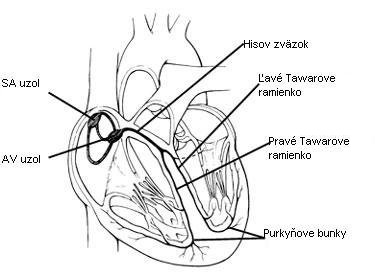
\includegraphics[scale=0.7]{48_img1_b}
\caption{Prevodový systém srdca}
\end{center}
\end{figure}

\newpage
\subsection{Akčný potenciál}
Ako vyrába a prenáša srdcové tkanivo elektrické impulzy? Aby sme si priebeh tohto deja mohli vysvetliť, musíme sa preniesť až na úroveň atómov.

\emph{Atóm je neutrálny,} ak má rovnaký počet protónov (kladne nabitých častíc) a elektrónov (záporne nabitých častíc). 

\emph{Ióny vznikajú} z elektricky neutrálnych atómov pridaním resp. ubraním elektrónov. 

V pokoji je srdcová bunka v \emph{polarizovanom stave}:
\begin{itemize}
	\item mimobunkový priestor je elektricky pozitívny pre vysokú koncentráciu kladných iónov sodíka a vápnika
	\item vnútrobunkový priestor je oproti vonkajšej strane negatívny
	\item rozdiel potenciálov je -90mV
\end{itemize}

Keď pokojový membránový potenciál dosiahne určitú prahovú hodnotu (cca. 15 mV), tzv. \emph{akčný potenciál}, tento pokojový stav sa náhle zmení. V membráne bunky sa otvoria prieduchy a kladne nabité ióny prúdia späť do bunky. Táto náhla strata polarizácie sa volá depolarizácia a vzniká pri nej elektrický prúd.

Po depolarizácii nastáva protikladný dej, repolarizácia, keď sa ióny znovu prečerpávajú von mimo membránu. Depolarizačná vlna vyvolávaná uzlom SA sa šíri po prevodovom systéme srdca a uvádza svaly do pohybu. Proces, ktorý začal pumpovaním iónov takto končí pumpovaním krvi. 

\begin{figure}[!ht]
\begin{center}
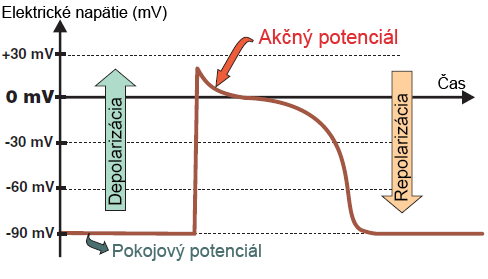
\includegraphics[scale=0.5]{action-potential-voltage}
\caption{Akčný potenciál v grafickom vyobrazení}
\end{center}
\end{figure}

%https://www.jfmed.uniba.sk/fileadmin/jlf/Pracoviska/ustav-patologickej-fyziologie/07Pregradualne_studium/01Vseobecne_lekarstvo/04Handouty_a_prednasky/01Handouty/01Elektrokardiografi1-jun10.pdf


\newpage 
\subsection{Prehľad prístrojov EKG}
\subsubsection{Druhy funkčných vyšetrení}
Elektrokardiografia je jedným zo základných lekárskych vyšetrení. Najčastejšie sa využíva v núdzových situáciách pri podozrení na srdcový infarkt, na zistenie poruchy súvisiacej s kardiovaskulárnym systémom alebo ako preventívne vyšetrenie so zámerom odhaliť možný srdcový defekt.

Vyšetrenie EKG je neinvazívne a nevyžaduje žiadnu špeciálnu prípravu. Pri klasickom EKG sa elektródy pripevnia na hrudník, zápästia a členky pacienta. Elektrické signály zachytené z povrchu tela, ktoré sú spravidla veľmi slabé, v rádoch milivoltov, prístroj zosilní a zaznamená. Následne ich lekár vyhodnotí.

Existuje niekoľko rôznych druhov vyšetrní:
\begin{itemize}
	\item \textbf{Štandardné 12-zvodové EKG} je najčastejšie používaný zo všetkých typov EKG. Pozostáva zo 6 končatinových zvodov a 6 hrudných zvodov. Každý zvod je samostatne zapisovaný na priebežne sa posunujúci špeciálny záznamový papier, prípadne zobrazuje hodnoty na monitore.
	\item \textbf{Záťažové EKG (ergometria)} ukáže správanie srdca a obehového systému pri námahovej aktivite. Na simuláciu sa väčšinou používa stacionárny bicykel alebo bežecký pás. Monitoruje sa záznam EKG v súvislosti s krvným tlakom. Na zázname sa pátra po zmenách, ktoré na EKG urobenom v pokoji nie sú viditeľné.
	\item \textbf{Dynamické EKG} umožňuje sledovať srdcovú činnosť pri bežných aktivitách počas 12-48 hodín. Zvýšením doby monitorovania sa zvyšuje pravdepodobnosť nálezu nepravidelností rytmu alebo námahových ischémií myokardu v zázname.
	\item \textbf{Tlakový Holter}. Ambulantné 24-hodinové sledovanie krvného tlaku je jednoduché vyšetrenie často indikované pri diagnostikovaní hypertenzie. Sníma sa tlak krvi v domácom prostredí pri každodenných činnostiach pomocou nafukovacej manžety.
\end{itemize}


\begin{figure}[!ht]
\begin{center}
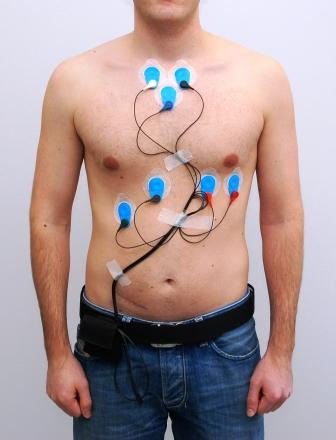
\includegraphics[scale=1]{holter}
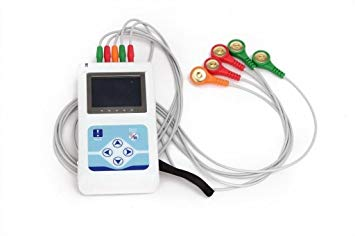
\includegraphics[scale=0.4]{portable-ecg}
\caption{Príprava pacienta na 24-48 hodinové monitorovanie a Holterov monitor}
\end{center}
\end{figure}

\newpage


\subsubsection{Časti klasického prístroja EKG}

\textbf{Tepelná tlačová hlava}
\\
Kreslí EKG krivku generovaním tepla.
\\
\\
\textbf{Termopapier}
\\
Prichádza do kontaktu s tlačovou hlavou. Na mieste dotyku sa farba papiera mení na čiernu, takto vzniká krivka EKG. Papier je tiež citlivý na tlak.
\\
\\
\textbf{Elektródy}
\\
Elektródy sú vyrobené z vodivého materiálu, ktorý dokáže zachytiť elektrické impulzy zo srdca. Signály odosielajú na spracovanie do meracieho prístroja cez pripojené káble.
\\
\\
\textbf{Zosilňovač}
\\
Zosilňovač je zariadenie, ktoré sa nachádza v elektrokardiografe a zvyšuje amplitúdu elektrického signálu. Signály prichádzajúce zo srdca sú relatívne slabé (0,0001V až 0,003V) a je potrebné ich zosilniť.
\\
\\
\textbf{Galvanometer}
\\
Premieňa prúd na mechanický pohyb.
\\
\\
\textbf{Sada EKG káblov}
\\
Slúžia na spojenie zvyčajne desiatich elektród s hlavnou jednotkou prístroja EKG. Takáto konfigurácia umožňuje monitorovať srdce z 12 ,,pohľadov".

\subsubsection{Výdobytky modernej elektrokardiografie}
Moderné prístroje EKG disponujú zabudovanými mikroprocesormi, ktoré ich riadia a rozširujú ich diagnostické schopnosti. Vďaka sofistikovaným matematickým algoritmom a modelom sú schopné previesť zložitú analýzu signálu a automaticky ho vyhodnotiť. Sú kompaktné, prenosné a vhodné i na monitorovanie mimo zdravotníckeho zariadenia.

Prepojiteľnosť s počítačom je v dnešnej dobe takmer samozrejmosťou, niektoré dokonca komunikujú bezdrôtovo a aj na diaľku. Digitalizácia údajov môže byť výhodná naporíklad z hľadiska archivácie alebo v prípade potreby zdieľať záznam so špecialistom.

Kardiologický monitor je častým rozšírením zariadenia EKG a umožňuje dlhodobo sledovať srdcovú aktivitu pacienta. Údaje zobrazuje v reálnom čase a ponúka náhľad kriviek ešte pred ich zápisom na papier.


\newpage

\subsection{Umiestnenie elektród}
Tri končatinové elektródy (pravá ruka, ľavá ruka, ľavá noha)  vytvárajú Einthovenov trojuholník. Vzniknú 3 \emph{bipolárne zvody} reprezentované stranami trojuholníka. Každý zvod pozostáva z dvoch elektród, z pozitívneho a z negatívneho. Pozitívny a negatívny pól spolu tvoria elektrický vektor, ktorý sa premieta na papier.

\begin{description}
	\item Zvod I: \tabto{1cm} $V_{I} = \phi_L - \phi_R$
	\item Zvod II: \tabto{1cm} $V_{II} = \phi_F - \phi_R$
	\item Zvod III:	\tabto{1cm} $V_{III} = \phi_F - \phi_L$
\end{description}
, kde: \\
\tabto{1cm} $V_{I}$ = napätie zvodu I\\
\tabto{1cm} $V_{II}$ = napätie zvodu II\\
\tabto{1cm} $V_{III}$ = napätie zvodu III\\
\tabto{1cm} $\phi_L$ = potenciál na ľavej ruke\\
\tabto{1cm} $\phi_R$ = potenciál na pravej ruke\\
\tabto{1cm} $\phi_F$ = potenciál na ľavej nohe\\
\\
Podľa Kirchhoffovho zákona platí, že veľkosť potenciálov (amplitúd na EKG zázname) v zvode $V_{II}$ je sumou potenciálov v zvodoch $V_{I}$ a  $V_{III}$:
\tabto{1cm} $V_{I} + V_{III} = V_{II}$
, z čoho vyplýva, že iba dva z troch zvodov sú nezávislé.
\\
\\
Einthoven definoval rozdiely potenciálov medzi troma pármi horeuvedených bodov ako základné končatinové zvody v elektrokardiografii.


\begin{figure}[!ht]
\begin{center}
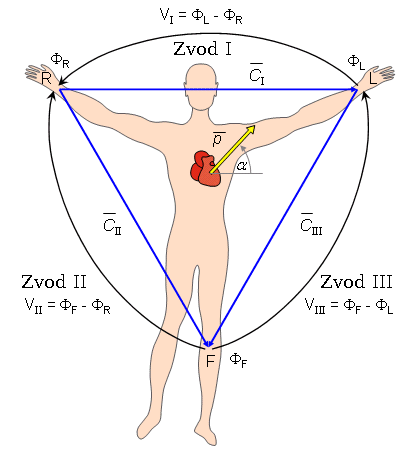
\includegraphics[scale=0.4]{ekg-zvody}
\caption{Einthovenove končatinové zvody a Einthovenov trojuholník}
\end{center}
\end{figure}
%http://www.bem.fi/book/15/15.htm


\subsection{Signál a jeho spracovanie}
Po úspešnom zmeraní a zosilnení signálu čelíme zložitej prekážke v snahe zachytiť srdcový rytmus. Signál je síce zosilnený, ale naďalej obsahuje mnoho nežiaducich elementov vplyvom rušivých faktorov z okolia. Výsledkom je skreslený biosignál, ktorý je v tejto fáze nepoužiteľný.

Nepresnosti v meraniach odborne nazývame \emph{artefakty}. Artefakty sa môžu prejavovať v menšej či väčšej miere v závislosti od nedokonalostí v priebehu vedenia signálu z pacienta do aparatúry (prístroja). V elektrokardiografii rozoznávame tri základné druhy artefaktov:
\begin{itemize}
	\item sieťový brum
	\item kolísanie nulovej línie (drift)
	\item myopotenciály
\end{itemize}

V minimalizácii nežiaduceho šumu nám napomáha súbor špecializovaných hardvérových i digitálnych filtrov.

\subsubsection{Sieťový brum}
Prvým krokom spracovania signálu je základná hardvérová filtrácia. Elektromagnetická interferencia (EMI) vzniká pôsobením  elektromagnetického poľa z elektrickej siete. Pri tomto jave dochádza k vzniku indukovaného napätia (Ui) a indukovaného prúdu na vodiči. Šum opísaného druhu môžeme charakterizovať pri frekvencii 50 Hz sínusového rušenia. Na potlačenie sieťového brumu je účinná kombinácia hardvérového RC článku s digitálnym filtrom. 

\subsubsection{Potlačenie driftu}
Drift alebo kolísanie nulovej línie opisuje skupinu elektrochemických a mechanických javov. Príkladmi elektrochemických sú potenie pod elektródami, nedostatočné odmastenie pokožky, malé množstvo kontaktného gélu. Dýchanie (do 0,8 Hz) a pomalé pohyby klienta (do 2 Hz) sú mechanické javy. Na odstránenie nízkofrekvenčnej rušivej zložky použijeme hornopriepustný filter.

\subsubsection{Myopotenciály}
Ďalší rušivý faktor pri vyšetrení EKG predstavuje svalová aktivita, najmä pri záťažovom EKG. Svaly počas pohybu vytvárajú elektrické impulzy, ktoré sa potom prejavujú vo forme muskuloskeletálneho artefaktu. Najväčším problémom v zdolaní účinku myopotenciálov je vzájomné prekrývanie frekvenčného pásma svalovej aktivity a užitočného pásma EKG. Na odstránenie tohto artefaktu nie je účinná pásmová priepusť. Vyžaduje sa pokročilejšie riešenie, napríklad pomocou adaptívnej filtrácie. 

\newpage
\subsubsection{Voľba filtrov}
\subsubsection*{Nekonečná impulzná odozva - IIR}
\subsubsection*{Konečná impulzná odozva - FIR}



\begin{figure}[!ht]
\begin{center}
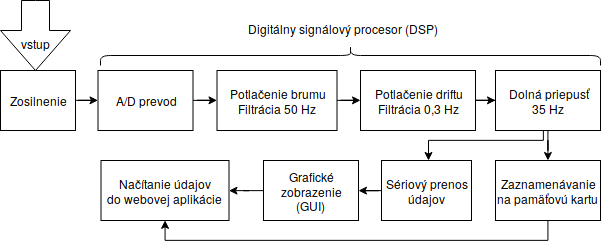
\includegraphics[scale=0.4]{flowchart}
\caption{Bloková schéma spracovania EKG}
\end{center}
\end{figure}

\newpage
\section{Návrh a konštrukcia hardvéru}
Proces návrhu hardvérových komponentov som si rozdelil do niekoľkých fáz kvôli systematickosti. Takýto spôsob práce mi umožnil priebežné testovanie a odhaľovanie možných chýb počas vývoja. Od začiatku až po finálny dizajn som prešiel tromi iteráciami projektu. 

Na návrh elektroniky a dizajn plošných spojov som používal grafický počítačový editor Eagle (verzia 9.1.3).

Prvý prototyp obvodu bol vyrobený podľa jednoduchej schémy. Pozostávala iba z jedného operačného zosilňovača a zopár rezistorov. Z bezpečnostných dôvodov bola namiesto laboratórneho zdroja použitá 9V batéria na napájanie obvodu. 

Operačný zosilňovač LM741 slúži na zosilnenie nízkonapäťového vstupu z elektród priložených na povrch tela. Je zapojený v diferenčnej konfigurácií, jeho invertujúci a neinvertujúci vstup predstavujú rozdielne napätia. Výstup je teda funkciou napäťovej diferencie medzi dvoma hrudnými elektródami. Faktor zisku je približne 50 podľa pomeru R5:R4. Z dôvodu, že zosilňovač funguje optimálne pre stredové hodnoty (medzi maximom a minimom), je nutné jeho vstupy dostať do použiteľného pásma. Na tento účel slúži napäťový delič R1-R2.

Analógový výstup bol pripojený do 3,5 mm mikrofónového rozhrania zvukovej karty počítača. Signál prešiel základnou softvérovou filtráciou a bol graficky zobrazovaný pomocou počítačovej aplikácie.

Hlavnou problematikou tohto návrhu bola všeobecná nespoľahlivosť a výskyt elektromagnetickej interferencie a iných artefaktov v meraných hodnotách.


\begin{figure}[!ht]
\begin{center}
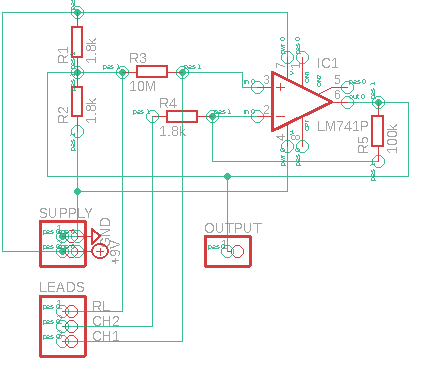
\includegraphics[scale=1]{schematic}
\caption{Schéma zosilňovacieho obvodu}
\end{center}
\end{figure}

Na minimalizáciu rušivých faktorov sa môže použiť pasívny RC dolnopriepustný filter.


Ďalším krokom je osamostatniť AD prevod signálu prostredníctvom mikrokontroléra. Aby sa to mohlo uskutočniť, zosilnený signál s negatívnou napäťovou zložkou sa musí premapovať  na rozsah kompatibilný s prevádzkovým rozsahom napätia mikrokontroléra.


\newpage
Srdcovú činnosť umožňujú malé elektrické impulzy, ktoré sa šíria po prevodovom systéme a pracovnom myokarde. Menia elektrické potenciály na rôznych bodoch pokožky približne o tisícinu voltu (1 mV). Táto elektrická aktivita v sebe skrýva neuveriteľné množstvo informácií, prostredníctvom ktorých môžeme získať náhľad do fungovania tohto zázračného orgánu.

K zachyteniu a odhaleniu signálu sa žiadne špeciálne vybavenie nevyžaduje. Odmerať ho dokážeme aj pomerne jednoduchým prístrojom.

Výzvou pokusu je spoľahlivo zosilniť a rozoznať pomerne slabý, milivoltový signál meniaci sa každú stotinu sekundy.

\newpage
\section*{Zoznam použitej literatúry}
\begin{itemize}
\item 1991. Ľudské telo - Komplexný sprievodca po ľudskom tele a jeho funkciách. Bratislava. GEMINI, spol. s.r.o. ISBN 80-85265-12-5.
\item IAIZZO, Paul A. 2005. Handbook of Cardiac Anatomy, Physiology, and Devices. New Jersey. Human Press, Inc. ISBN 1-59259-835-8.
\item HANÁČEK, Ján, PLEVKOVÁ, Jana. 2009. Elektrokardiografia - Základné mechanizmy porúch elektrickej funkcie srdca a ich manifestácia na Ekg krivke. Martin. Ústav patologickej fyziológie JLF UK.
\item MALMIVUO, Jaakko, PLONSEY, Robert. 1995. Bioelectromagnetism - Principles and Applications of Bioelectric and Biomagnetic Fields. Oxford. Oxford University Press.
\item BÓRIKOVÁ, Ivana. 2016. Funkčné vyšetrenie respiračného, kardiovaskulárneho a močového systému. Portál Jesseniovej lekárskej fakulty Univerzity Komenského. ISSN 1337-7396.
\item MIŠČÍK, Peter. 2011. Zpracování elektrokardiogramu. Vysoké učení technické v Brně. 
\item www.kardiolog.sk/o-srdci/
\item www.techmed.sk/akcny-potencial/
\item www.wikiskripta.eu/w/Rušení\_biosignálů\_a\_artefakty
\item www.swharden.com/wp/2016-08-08-diy-ecg-with-1-op-amp/
\item www.arduino.cc/en/Tutorial/ArduinoToBreadboard
\item images-na.ssl-images-amazon.com/images/I/51jDS6PVO6L.\_SX355\_.jpg
\item cardiocenter.az/uploads/posts/2017-06/1498069942\_4-holter.jpg
\item github.com/tttapa/Filters
\end{itemize}


\end{document}